%%%%%%%%%%%%%%%%%%%%%%%%%%%%%%%%%%%%%%%%%
% HW Template
% LaTeX Template
% Version 1.0 (19/10/18)
% Modified by
% Erdem TUNA
% Halil TEMURTAŞ 
% Enes TAŞTAN 
%%%%%%%%%%%%%%%%%%%%%%%%%%%%%%%%%%%%%%%%%
%
%----------------------------------------------------------------------------------------
%	PACKAGES AND OTHER DOCUMENT CONFIGURATIONS
%----------------------------------------------------------------------------------------
\documentclass[a4paper,12pt]{article}
%-----packages------
\usepackage[a4paper, total={6.2in, 8.5in}]{geometry}
\usepackage[english]{babel}
\usepackage[utf8x]{inputenc}
\usepackage{amsmath}
\usepackage{mathtools}
\usepackage{graphicx}
\usepackage[colorinlistoftodos]{todonotes}
\usepackage{gensymb} % this could be problem
\usepackage{float}
\usepackage{fancyref}
\usepackage{subcaption}
\usepackage[toc,page]{appendix} %appendix package
\usepackage{xcolor}
\usepackage{listings}
\usepackage{xspace}
\usepackage{amssymb}
\usepackage{nicefrac}
\usepackage{gensymb}
\usepackage{fancyhdr}
\usepackage{blindtext}  % for dummy text, use \blindtext or \BlindText
\usepackage{lipsum}    % for dummy text, use \lipsum[3-56]
\usepackage[final]{pdfpages}  % pdf include
\usepackage{array} %allows more options in tables
\usepackage{pgfplots,pgf,tikz} %coding plots in latex
\usepackage{capt-of} % allows caption outside the figure environment
\usepackage[export]{adjustbox} %more options for adjusting the images
\usepackage{multicol,multirow,slashbox} % allows tables like table1
%\usepackage[hyperfootnotes=false]{hyperref} % clickable references
\usepackage{epstopdf} % useful when matlab is involved
%\usepackage{placeins} % prevents the text after figure to go above figure with \FloatBarrier 
%\usepackage{listingsutf8,mcode} %import .m or any other code file mcode is for matlab highlighting

%-----end of packages

%-----specifications-----
\definecolor{mGreen}{rgb}{0,0.6,0} % for python
\definecolor{mGray}{rgb}{0.5,0.5,0.5}
\definecolor{mPurple}{rgb}{0.58,0,0.82}
\definecolor{mygreen}{RGB}{28,172,0} % color values Red, Green, Blue for matlab
\definecolor{mylilas}{RGB}{170,55,241}

\setcounter{secnumdepth}{5} % how many sectioning levels to assign numbers to
\setcounter{tocdepth}{5}    % how many sectioning levels to show in ToC

\lstdefinestyle{CStyle}{
	commentstyle=\color{mGreen},
	keywordstyle=\color{magenta},
	numberstyle=\tiny\color{mGray},
	stringstyle=\color{mPurple},
	basicstyle=\footnotesize,
	breakatwhitespace=false,         
	breaklines=true,
	frame=single,
	rulecolor=\color{black!40},                 
	captionpos=b,                    
	keepspaces=true,                 
	numbers=left,                    
	numbersep=5pt,                  
	showspaces=false,                
	showstringspaces=false,
	showtabs=false,                  
	tabsize=2,
	language=C
}

\lstset{language=Matlab,%
	%basicstyle=\color{red},
	breaklines=true,%
	frame=single,
	rulecolor=\color{black!40},
	morekeywords={matlab2tikz},
	keywordstyle=\color{blue},%
	morekeywords=[2]{1}, keywordstyle=[2]{\color{black}},
	identifierstyle=\color{black},%
	stringstyle=\color{mylilas},
	commentstyle=\color{mygreen},%
	showstringspaces=false,%without this there will be a symbol in the places where there is a space
	numbers=left,%
	numberstyle={\tiny \color{black}},% size of the numbers
	numbersep=9pt, % this defines how far the numbers are from the text
	emph=[1]{for,end,break},emphstyle=[1]\color{red}, %some words to emphasise
	%emph=[2]{word1,word2}, emphstyle=[2]{style},    
}


\tikzset{
	desicion/.style={
		diamond,
		draw,
		text width=4em,
		text badly centered,
		inner sep=0pt
	},
	block/.style={
		rectangle,
		draw,
		text width=10em,
		text centered,
		rounded corners
	},
	cloud/.style={
		draw,
		ellipse,
		minimum height=2em
	},
	descr/.style={
		fill=white,
		inner sep=2.5pt
	},
	connector/.style={
		-latex,
		font=\scriptsize
	},
	rectangle connector/.style={
		connector,
		to path={(\tikztostart) -- ++(#1,0pt) \tikztonodes |- (\tikztotarget) },
		pos=0.5
	},
	rectangle connector/.default=-2cm,
	straight connector/.style={
		connector,
		to path=--(\tikztotarget) \tikztonodes
	}
}

\tikzset{
	desicion/.style={
		diamond,
		draw,
		text width=4em,
		text badly centered,
		inner sep=0pt
	},
	block/.style={
		rectangle,
		draw,
		text width=10em,
		text centered,
		rounded corners
	},
	cloud/.style={
		draw,
		ellipse,
		minimum height=2em
	},
	descr/.style={
		fill=white,
		inner sep=2.5pt
	},
	connector/.style={
		-latex,
		font=\scriptsize
	},
	rectangle connector/.style={
		connector,
		to path={(\tikztostart) -- ++(#1,0pt) \tikztonodes |- (\tikztotarget) },
		pos=0.5
	},
	rectangle connector/.default=-2cm,
	straight connector/.style={
		connector,
		to path=--(\tikztotarget) \tikztonodes
	}
}
%-----end of specifications-----


%----commands----
\newcommand\nd{\textsuperscript{nd}\xspace}
\newcommand\rd{\textsuperscript{rd}\xspace}
\newcommand\nth{\textsuperscript{th}\xspace} %\th is taken already
\newcommand{\specialcell}[2][c]{ \begin{tabular}[#1]{@{}c@{}}#2\end{tabular}} % for too long table lines

\newcommand{\blankpage}{
	\- \\[9cm]	
	{ \centering \textit{This page intentionally left blank.} \par }
	\- \\[9cm]
}% For Blank Page

\makeatletter
\renewcommand\paragraph{\@startsection{paragraph}{4}{\z@}%
	{-2.5ex\@plus -1ex \@minus -.25ex}%
	{1.25ex \@plus .25ex}%
	{\normalfont\normalsize\bfseries}}
\makeatother
%-----end of commands-----


\pagestyle{fancy}
\fancyhead[LO,LE]{Halil TEMURTAŞ / 2094522   }
\fancyhead[RO,RE]{November 23,2018}
\fancyfoot[RO,RE]{
\includegraphics[width=2.7cm]{images/eelogo}}

\begin{document}
\begin{center}
	\textbf{\large EE402 Discrete Time Systems \\[0.2cm] MP-5} \\
\end{center}


\begin{enumerate}
	\item To easy the design process, the Tustin transform will be used throughout this mini-project.
		
		
	
	\lstinputlisting[language=Matlab,firstline=10, lastline=21]{MP5.m}
	
	\begin{figure}[H]
			\center
			\setlength{\unitlength}{\textwidth} 
		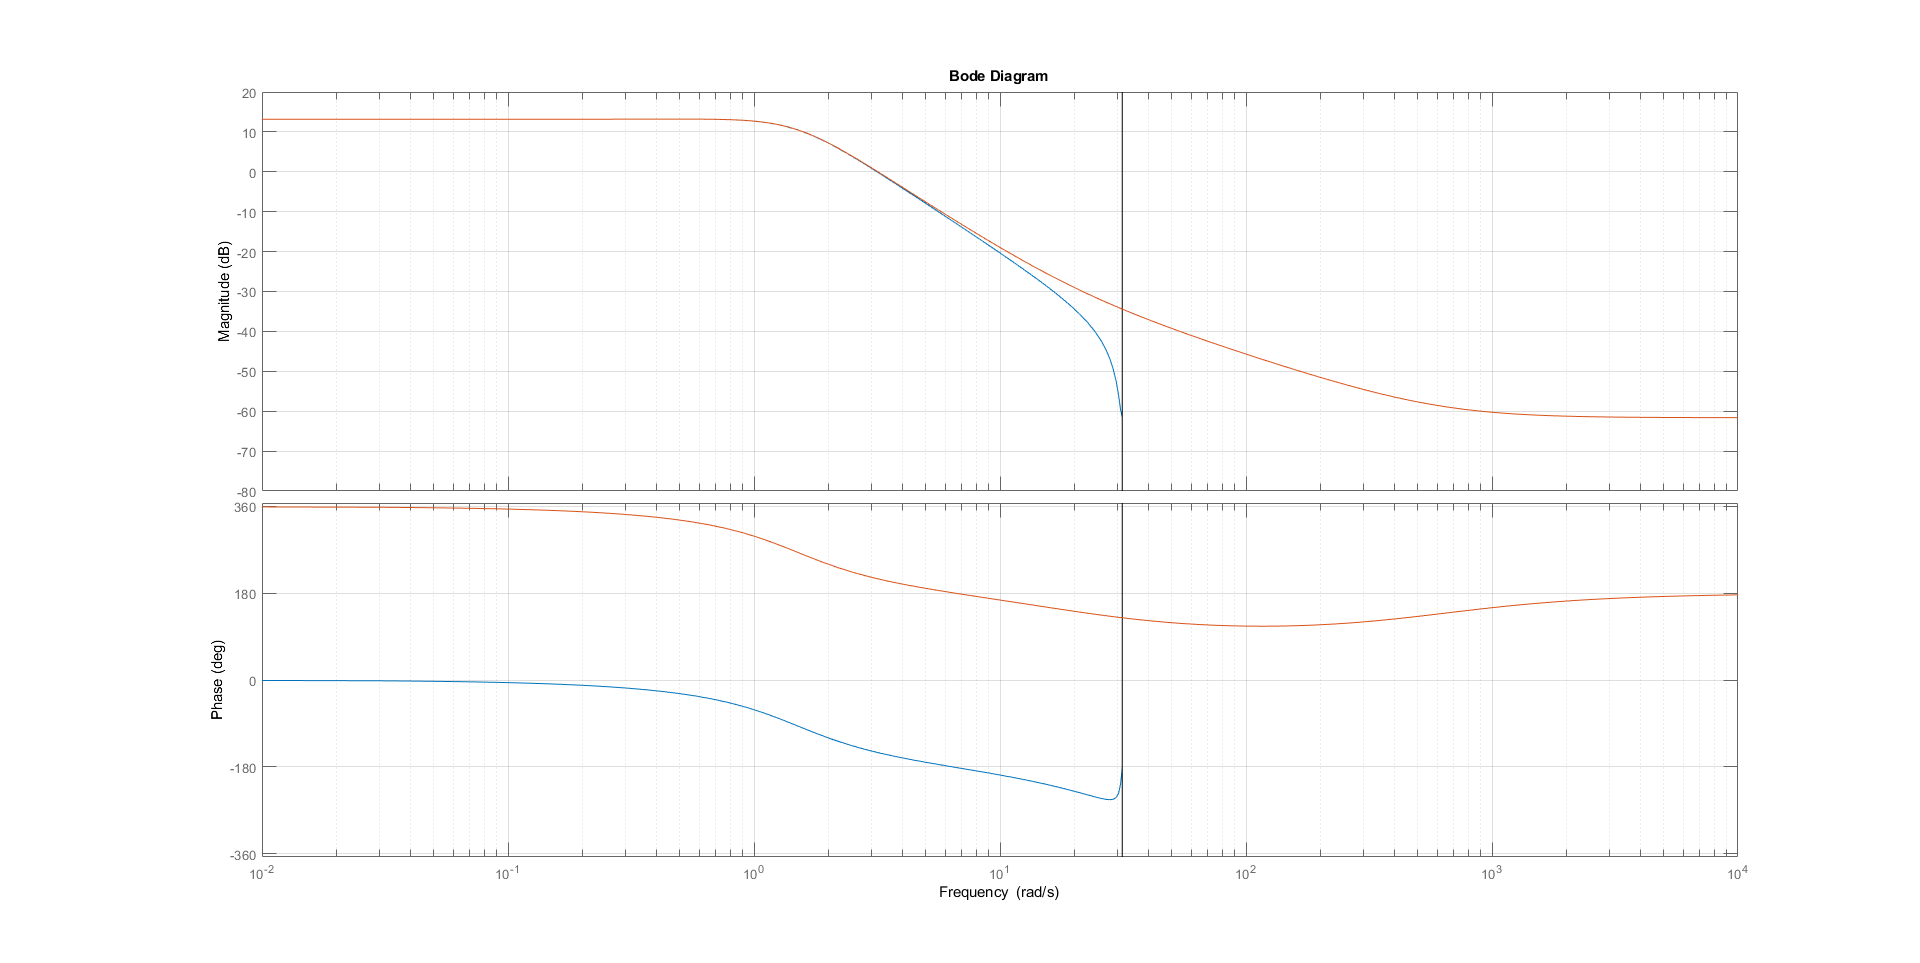
\includegraphics[width=1.0\unitlength]{images/a1}
  		\caption{\label{fig:a}Bode Plot of Discrete TF and of its Tustin Transform }
	\end{figure}
	
	Let us now find the uncompensated phase margin for T=1. 
	
	\begin{figure}[H]
			\center
			\setlength{\unitlength}{\textwidth} 
		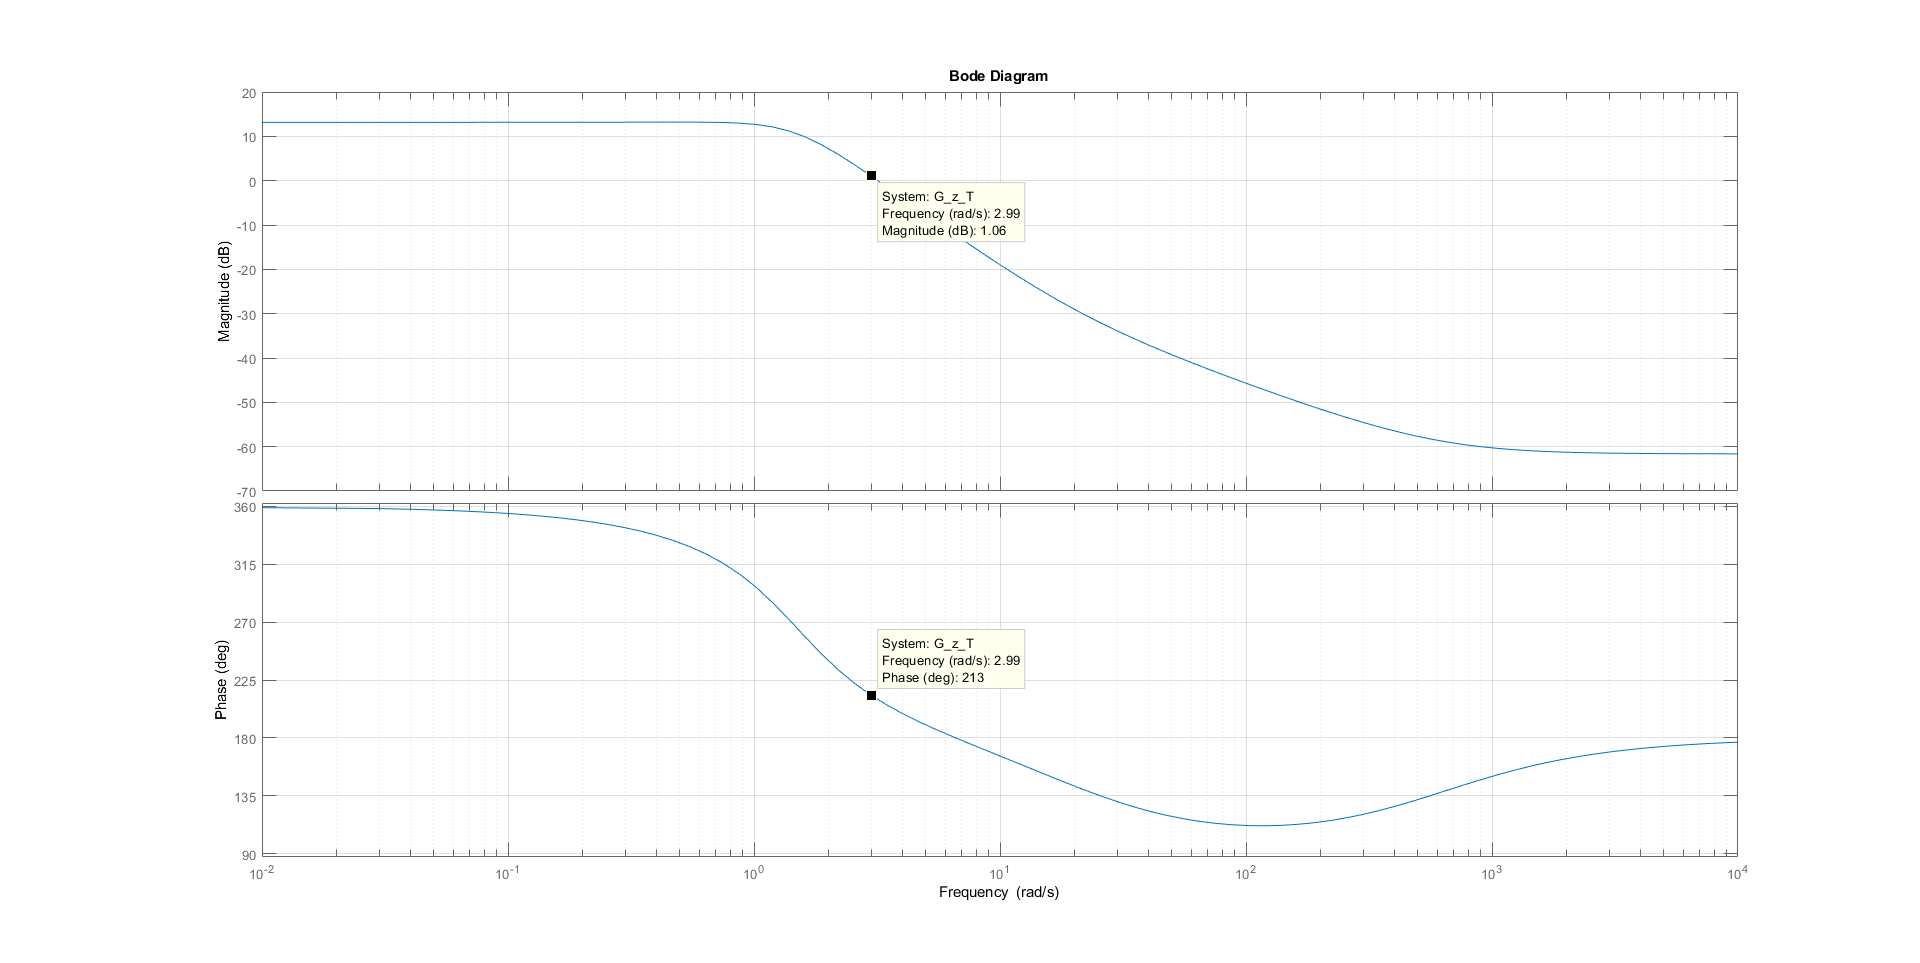
\includegraphics[width=1.0\unitlength]{images/c}
  		\caption{\label{fig:c}-}
	\end{figure}
	
	As can be seen from the \textit{Figure~\ref{fig:c}} that the $ PM \approx 29$.
	
	
	for desired $PM=[10,15]$
	
	$$ \Delta PM \approx [-19,-14] $$
	
	For negative phase margin, let us use the following compensator type
	
	$$ G_C(s)=\cfrac{1}{K_{Lead}\cfrac{T_Las+1}{Tl/as+1}} $$
	
	After trying couple of compensator bode plot for T=1 and varying a's. $ a=1.6 $ seems like a good choice. The bode plot for a compensator with $a=1.6$ can be seen at \textit{Figure~\ref{fig:d}} 
	
	\begin{figure}[H]
			\center
			\setlength{\unitlength}{\textwidth} 
		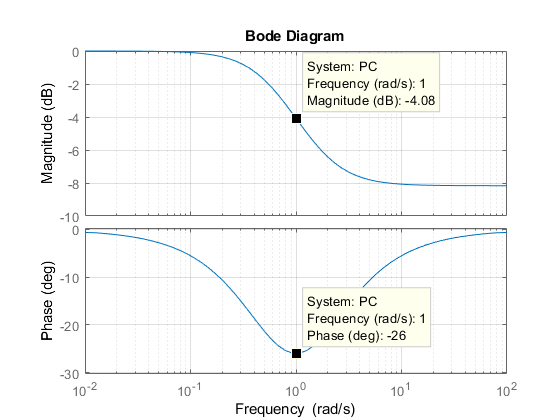
\includegraphics[width=0.75\unitlength]{images/desired_a1}
  		\caption{\label{fig:d}Bode plot for a compensator with $a=1.6$}
	\end{figure}
	
	To find the proper $T_L$ value, the bode plot of the uncompensated system was investigated. At a frequency of $w_x=4\ rad/sec$, the system has a gain of
	
	$$ 20log_{10}(1/a) = -4.08$$
	
	Thus;
	
	$$ T_L=1/w_x=1/4=0.25 $$
	
	\begin{figure}[H]
			\center
			\setlength{\unitlength}{\textwidth} 
		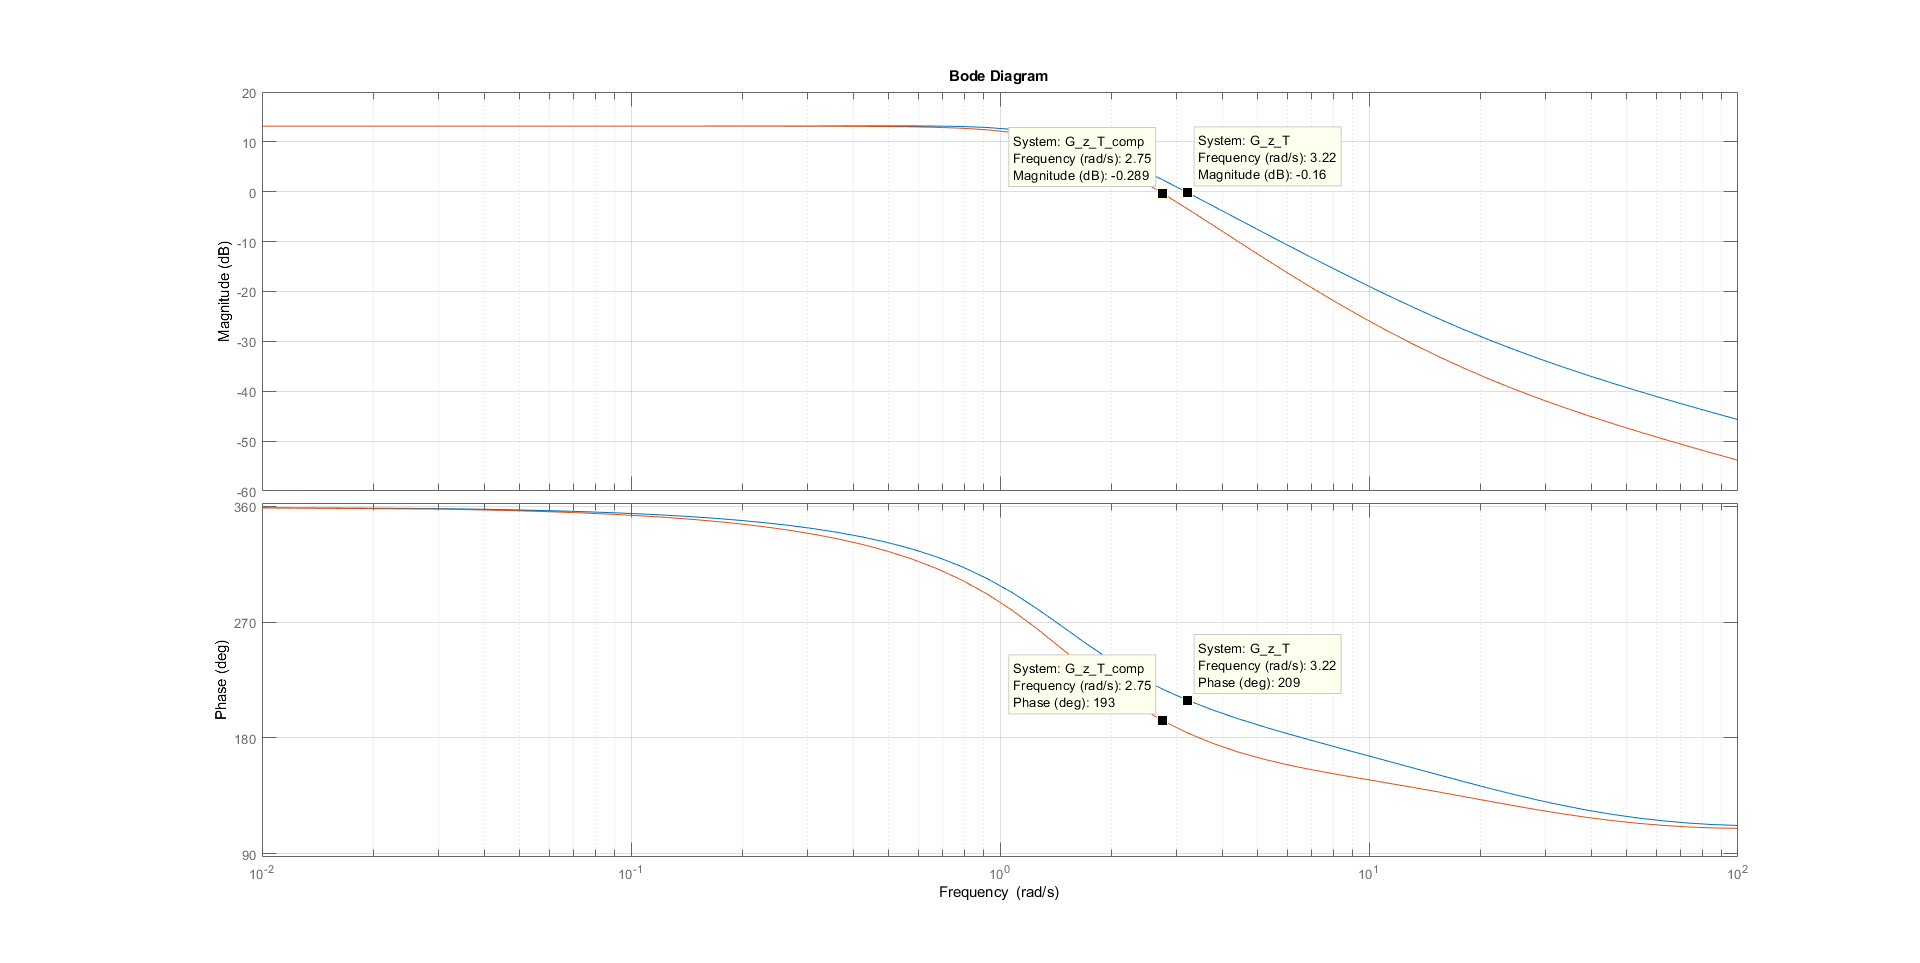
\includegraphics[width=1.0\unitlength]{images/comped1}
  		\caption{\label{fig:e}Bode Plots of compensated and uncompensated system}
	\end{figure}
	
	From the bode plots at \textit{Figure~\ref{fig:d}}, it can be observed that th new compensated system has a phase margin of 13 degree which is desired region.
	
	\begin{figure}[H]
			\center
			\setlength{\unitlength}{\textwidth} 
		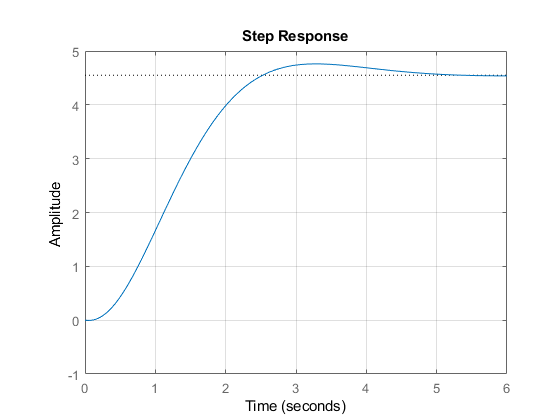
\includegraphics[width=0.75\unitlength]{images/comped1_step}
  		\caption{\label{fig:f} Step Response of the compensated system }
	\end{figure}
	
	Thus, the compensator can be designed to be as
	
	$$ G_C(s)=\cfrac{1}{K_{Lead}\cfrac{T_Las+1}{Tl/as+1}} $$
	$$ K_{Lead}=1 $$
	$$ TL=0.25$$
	$$ a=1.6$$
	
	\item for $PM=[25,30]$
	
	
	$$ \Delta PM \approx [-4,1] $$
	
	Following the similar steps, choosing $ a=1.1 $ seems good,  
	
	\begin{figure}[H]
			\center
			\setlength{\unitlength}{\textwidth} 
		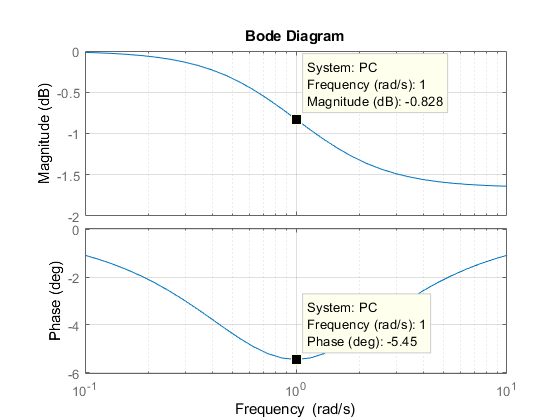
\includegraphics[width=1.0\unitlength]{images/desired_a}
  		\caption{\label{fig:10}Bode plot for a compensator with $a=1.1$}
	\end{figure}
	
	$$ T_L=1/2.82.=0.35 $$
	
	\begin{figure}[H]
			\center
			\setlength{\unitlength}{\textwidth} 
		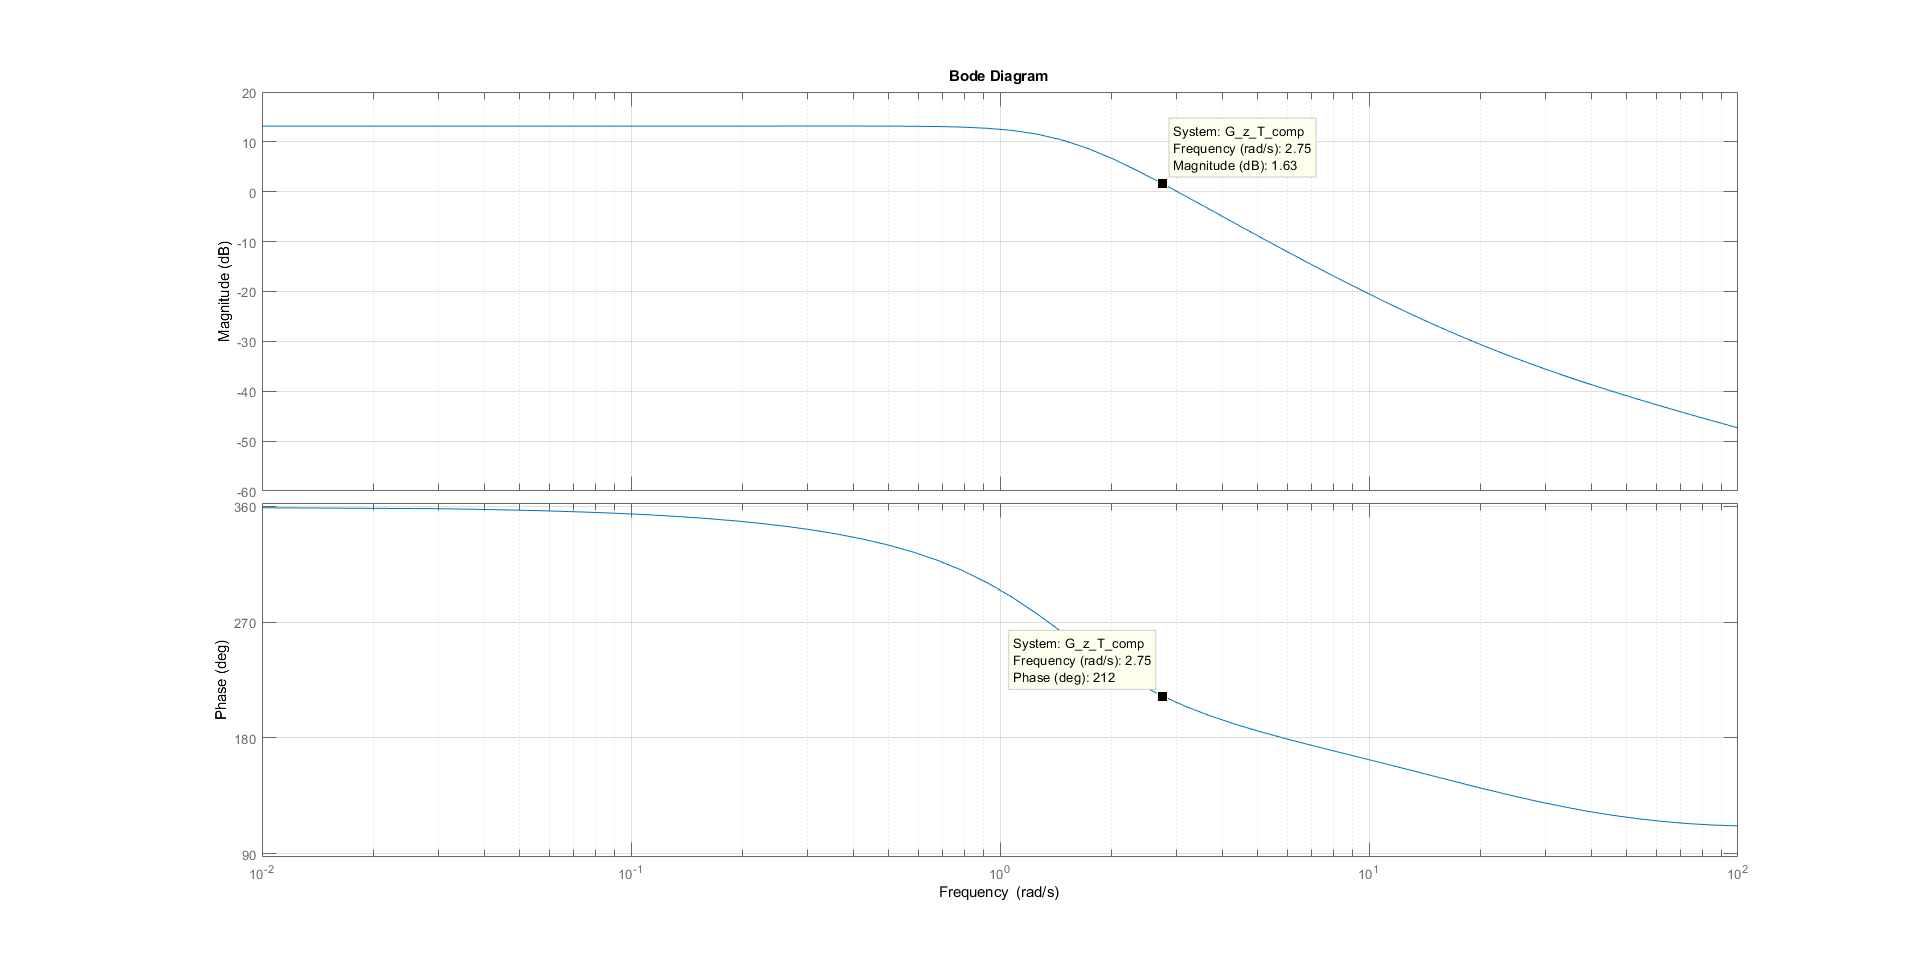
\includegraphics[width=1.0\unitlength]{images/comped2b}
  		\caption{\label{fig:k}Bode Plots of compensated system}
	\end{figure}
	
	\begin{figure}[H]
			\center
			\setlength{\unitlength}{\textwidth} 
		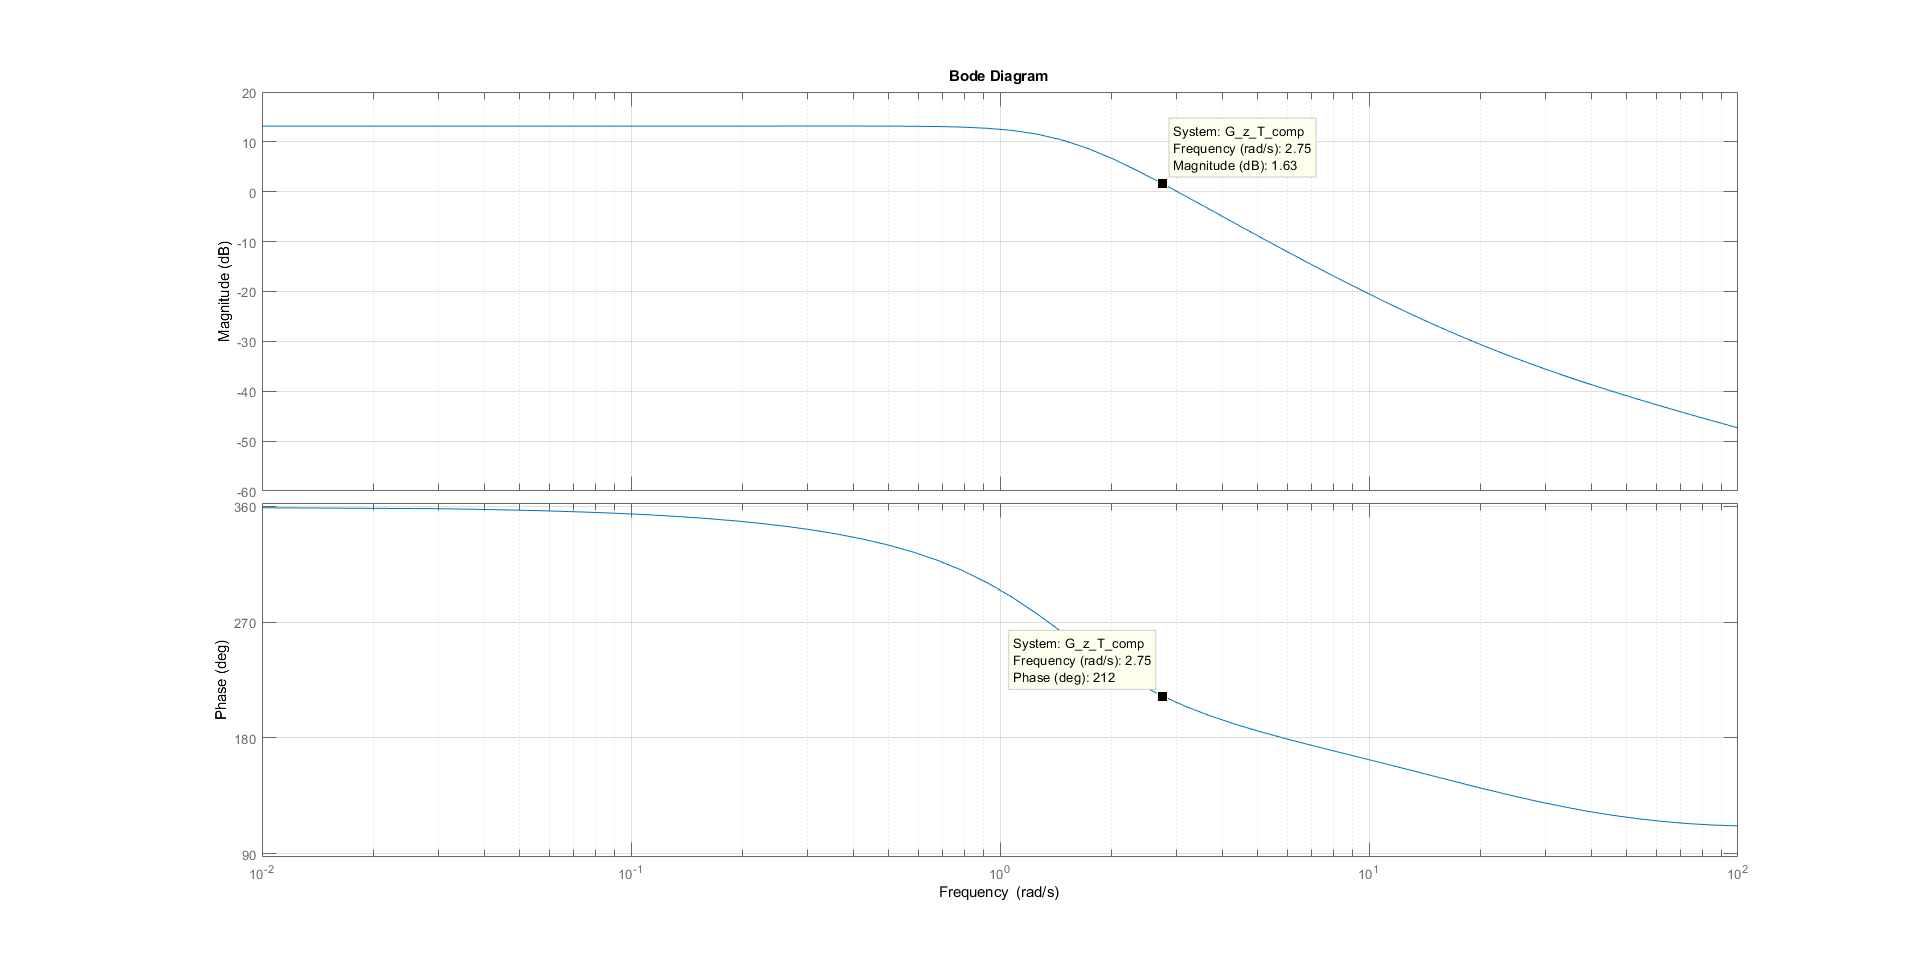
\includegraphics[width=1.0\unitlength]{images/comped2b}
  		\caption{\label{fig:l}Bode Plots of compensated and uncompensated system}
	\end{figure}
	
	From \textit{Figures~\ref{fig:k} and \ref{fig:l}}, the new phase margin for compansated system can be approximately found to be as 28 degree degree.
	
	\begin{figure}[H]
			\center
			\setlength{\unitlength}{\textwidth} 
		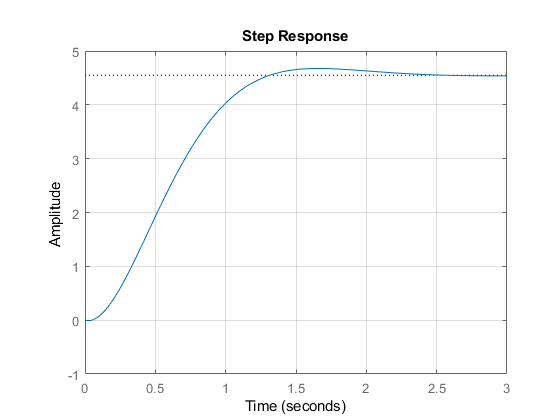
\includegraphics[width=0.75\unitlength]{images/comped2_step}
  		\caption{\label{fig:10}Step Response of the compensated system}
	\end{figure}
	
	Thus, the compensator can be designed to be as
	
	$$ G_C(s)=1\cfrac{1}{K_{Lead}\cfrac{T_Las+1}{Tl/as+1}} $$
	$$ K_{Lead}=1 $$
	$$ TL=0.35$$
	$$ a=1.1$$
	
	

	\begin{figure}[H]
			\center
			\setlength{\unitlength}{\textwidth} 
		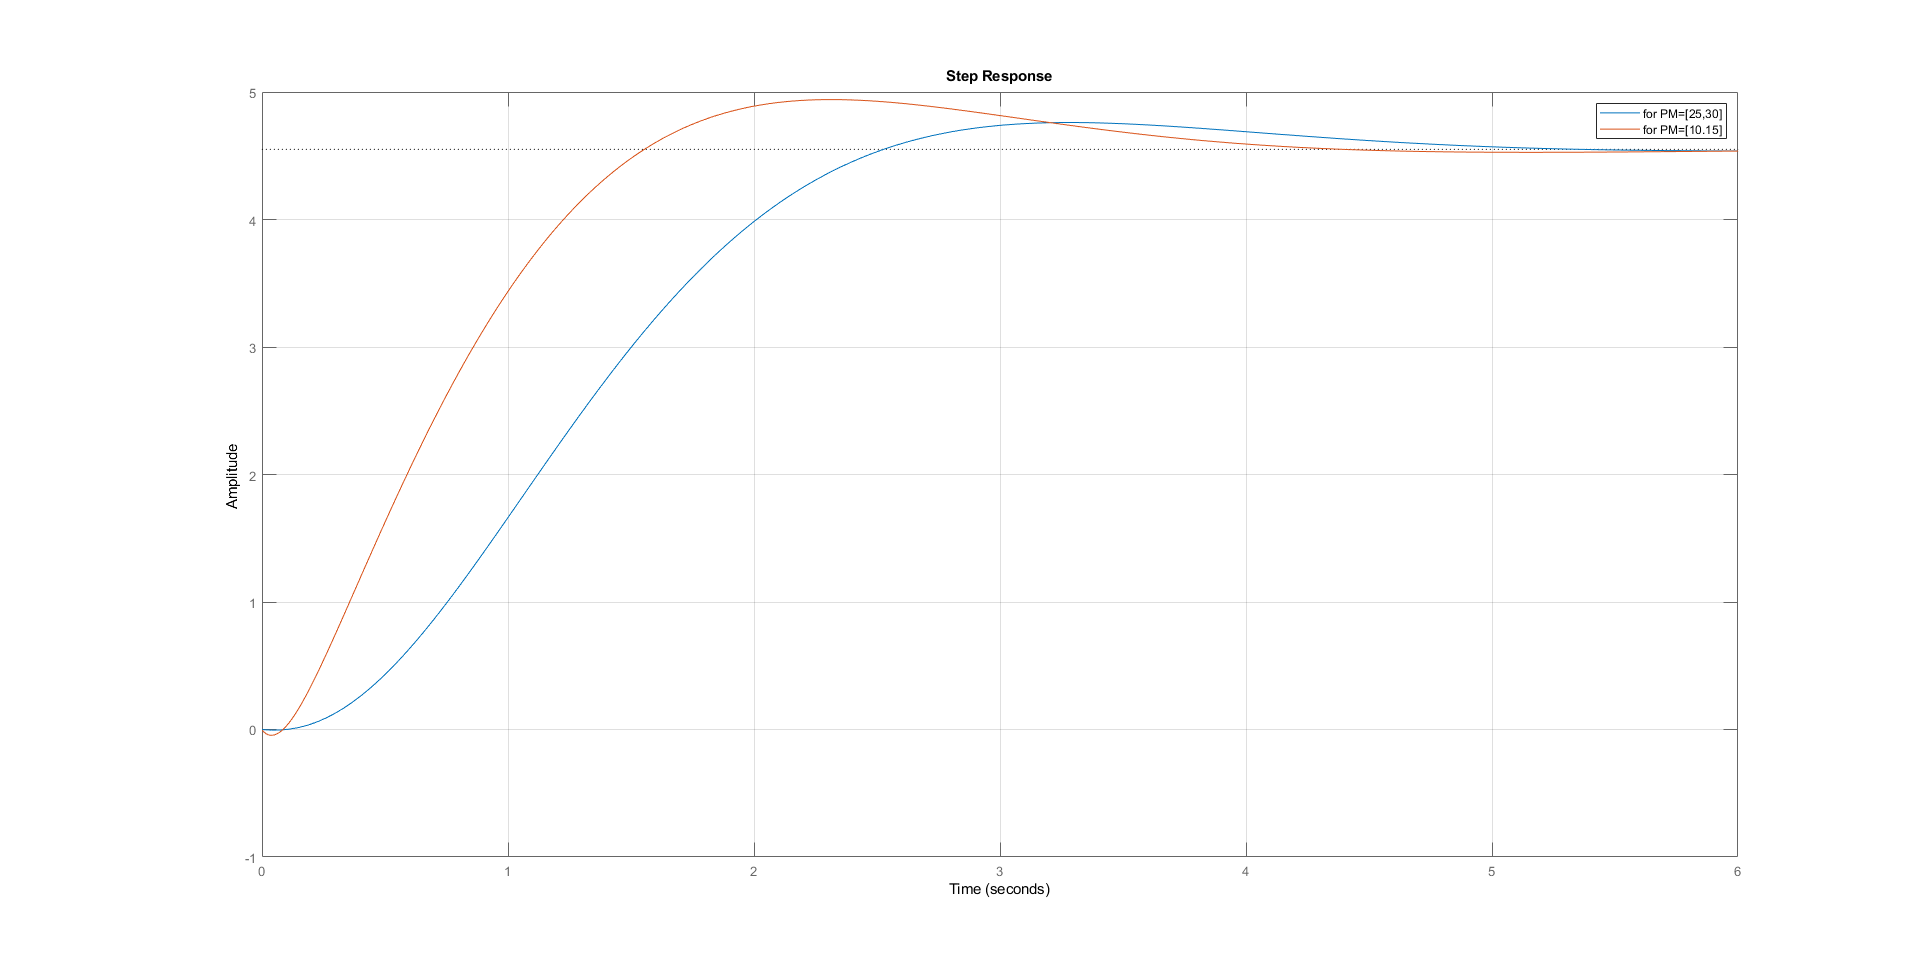
\includegraphics[width=0.75\unitlength]{images/step_t1}
  		\caption{\label{fig:10} Difference in Step Responses of both compensated systems}
	\end{figure}
	
	As the phase margin is decreased the settling time is increased, the overshoot decreased. The steady state error stayed same.
	
	\item T=0.5
	
	\begin{figure}[H]
			\center
			\setlength{\unitlength}{\textwidth} 
		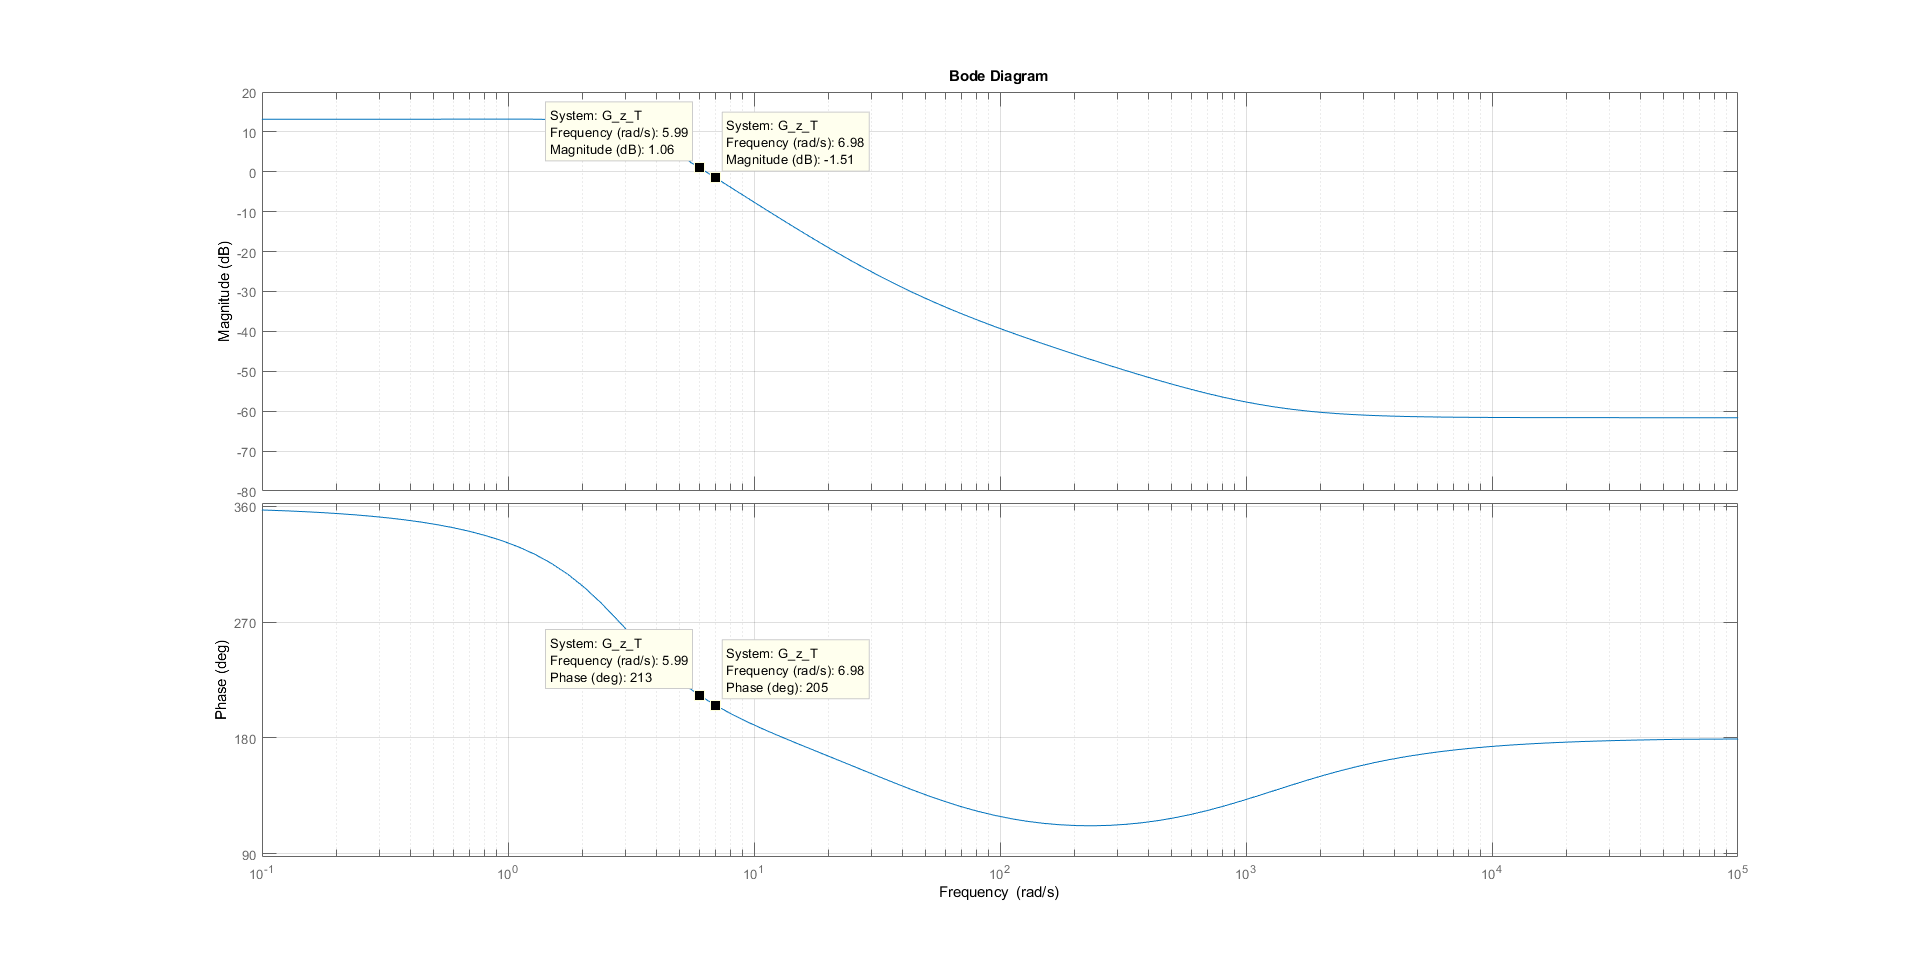
\includegraphics[width=1.0\unitlength]{images/uncomped}
  		\caption{\label{fig:10}-}
	\end{figure}
	
	$$ PM \approx 30$$
	
	
	for $PM=[10,15]$
	
	$$ \Delta PM \approx [-20,-15] $$
	
	Choose $ a=1.55 $ seems good,  
	
	$$ T_L=1/4=0.24 $$
	
	\begin{figure}[H]
			\center
			\setlength{\unitlength}{\textwidth} 
		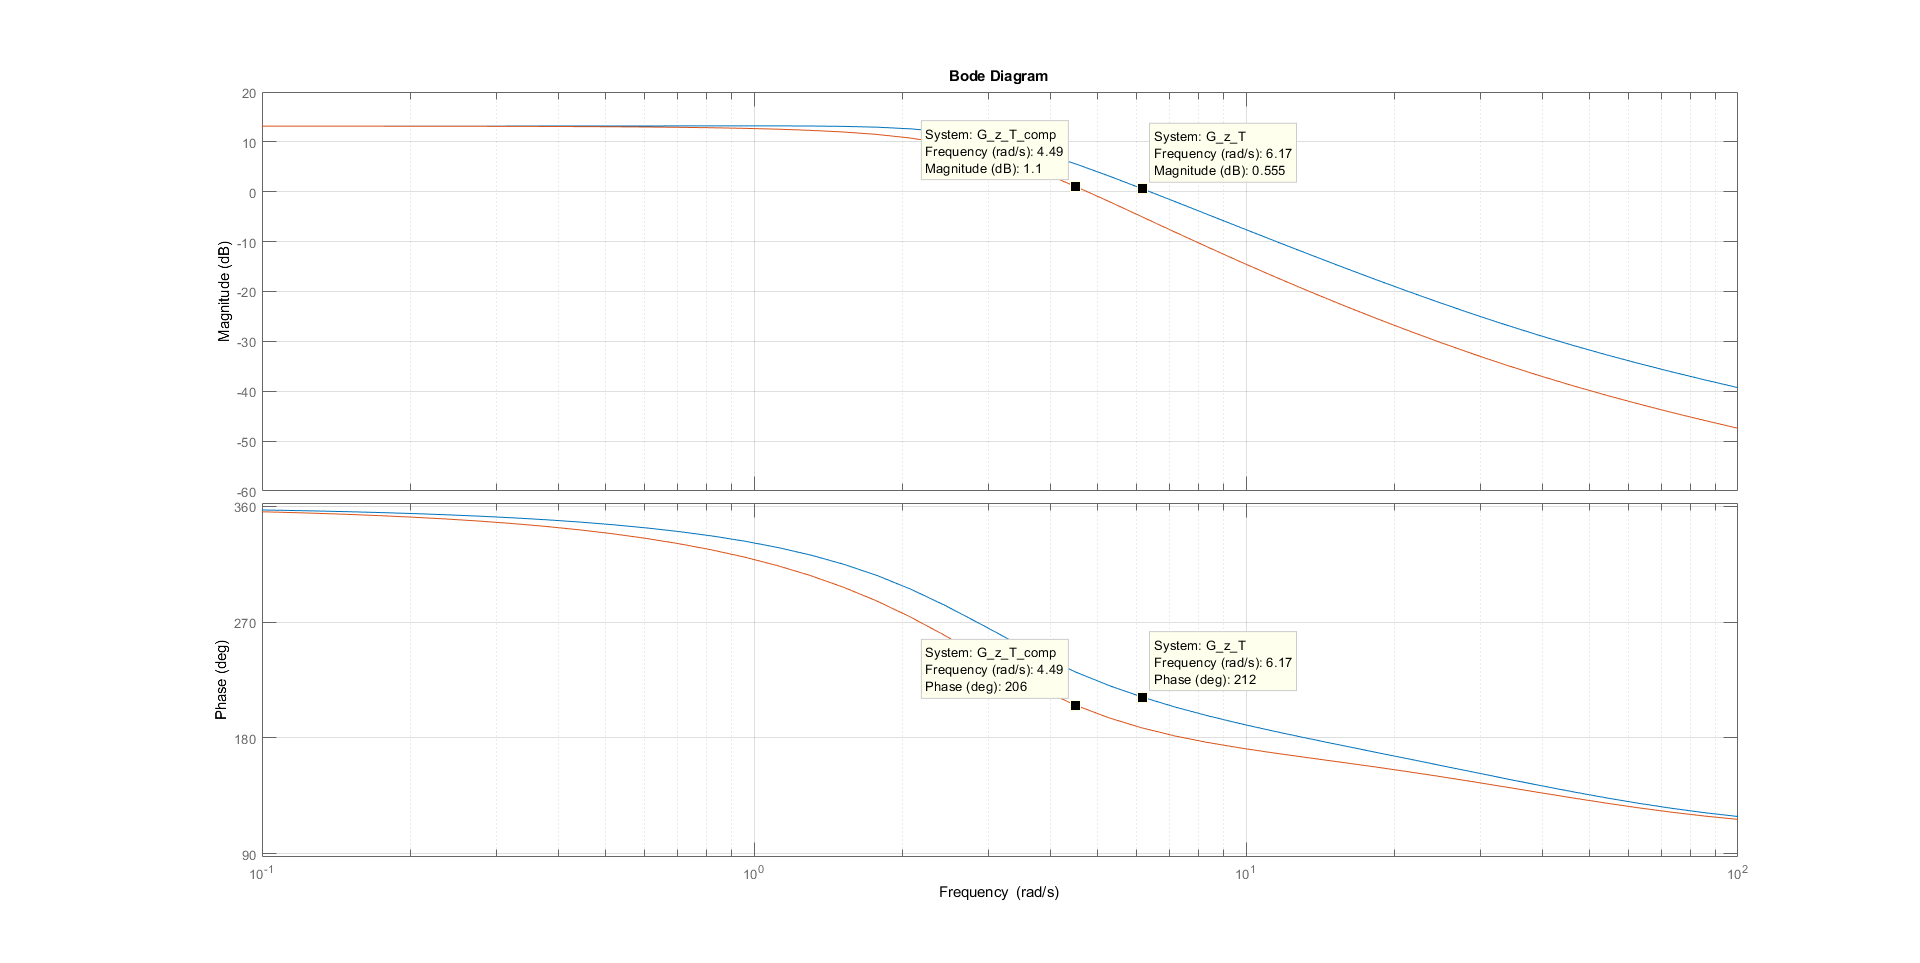
\includegraphics[width=1.0\unitlength]{images/compedb1}
  		\caption{\label{fig:10}Bode Plots of compensated and uncompensated system}
	\end{figure}
	
	New phase margin is 14 degree
	
	\begin{figure}[H]
			\center
			\setlength{\unitlength}{\textwidth} 
		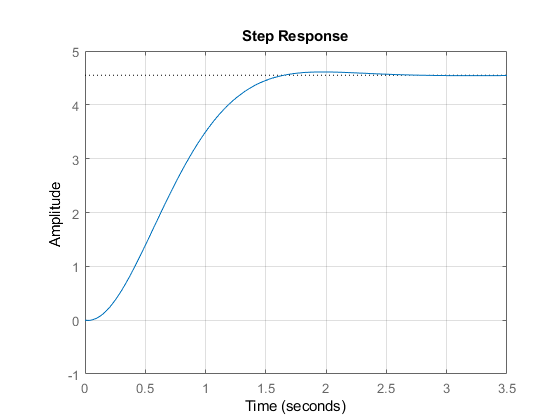
\includegraphics[width=0.75\unitlength]{images/comped1b_step}
  		\caption{\label{fig:10}Step Response of the compensated system}
	\end{figure}
	
	$$ G_C(s)=1\cfrac{1}{K_{Lead}\cfrac{T_Las+1}{Tl/as+1}} $$
	$$ K_{Lead}=1 $$
	$$ TL=0.24$$
	$$ a=1.55$$
	
	\item for $PM=[25,30]$
	
	
	$$ \Delta PM \approx [-5,0] $$
	
	Choose $ a=1.14 $ seems good,  
	
	
	$$ T_L=0.37 $$
	
	\begin{figure}[H]
			\center
			\setlength{\unitlength}{\textwidth} 
		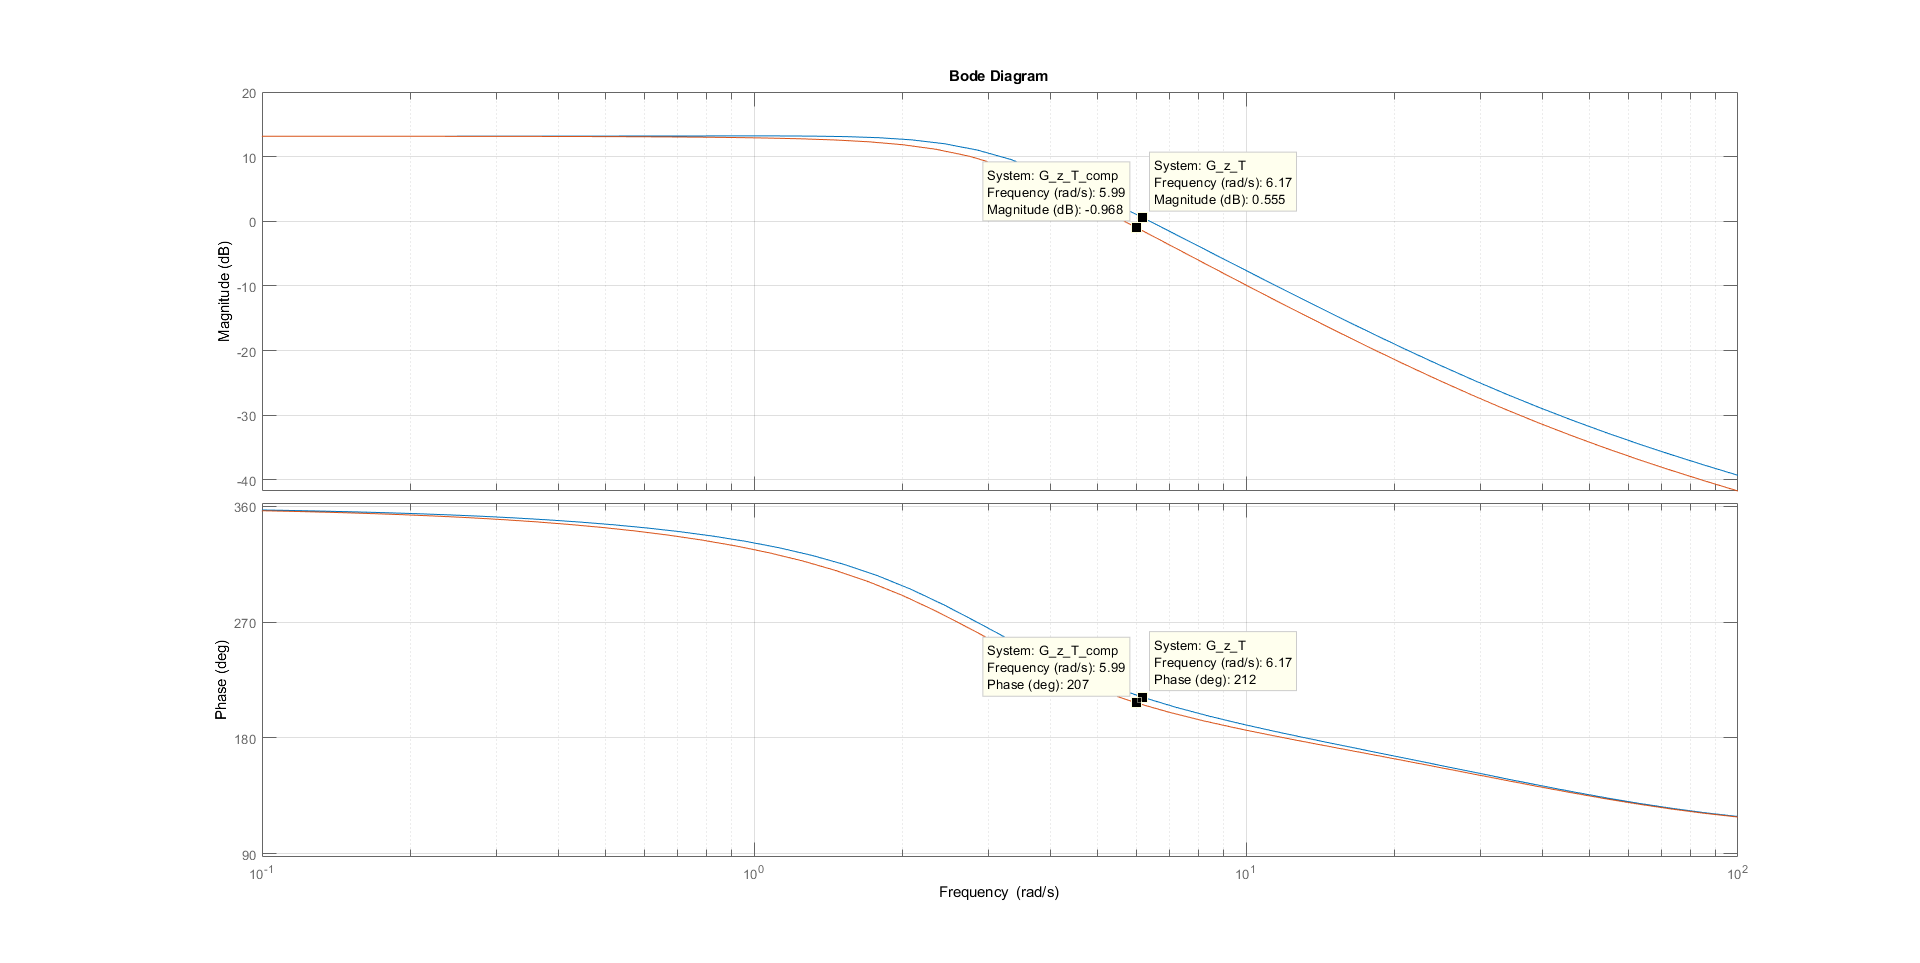
\includegraphics[width=1.0\unitlength]{images/compedb2}
  		\caption{\label{fig:10}Bode Plots of compensated and uncompensated system}
	\end{figure}
	
	
	New phase margin is approximately 29 degree degree
	
	\begin{figure}[H]
			\center
			\setlength{\unitlength}{\textwidth} 
		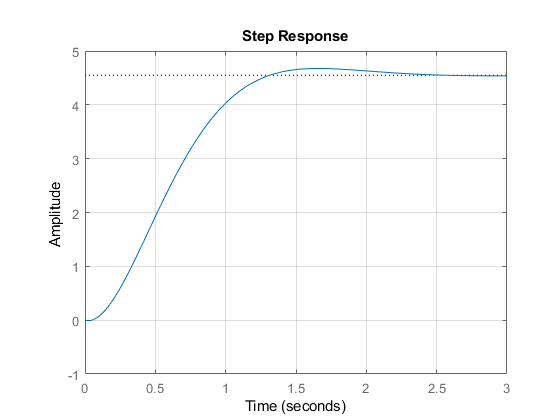
\includegraphics[width=0.75\unitlength]{images/comped2_step}
  		\caption{\label{fig:10}Step Response of the compensated system}
	\end{figure}
	
	$$ G_C(s)=1\cfrac{1}{K_{Lead}\cfrac{T_Las+1}{Tl/as+1}} $$
	$$ K_{Lead}=1 $$
	$$ TL=0.37$$
	$$ a=1.14$$
	
	

	\item -
	
	
	\begin{figure}[H]
			\center
			\setlength{\unitlength}{\textwidth} 
		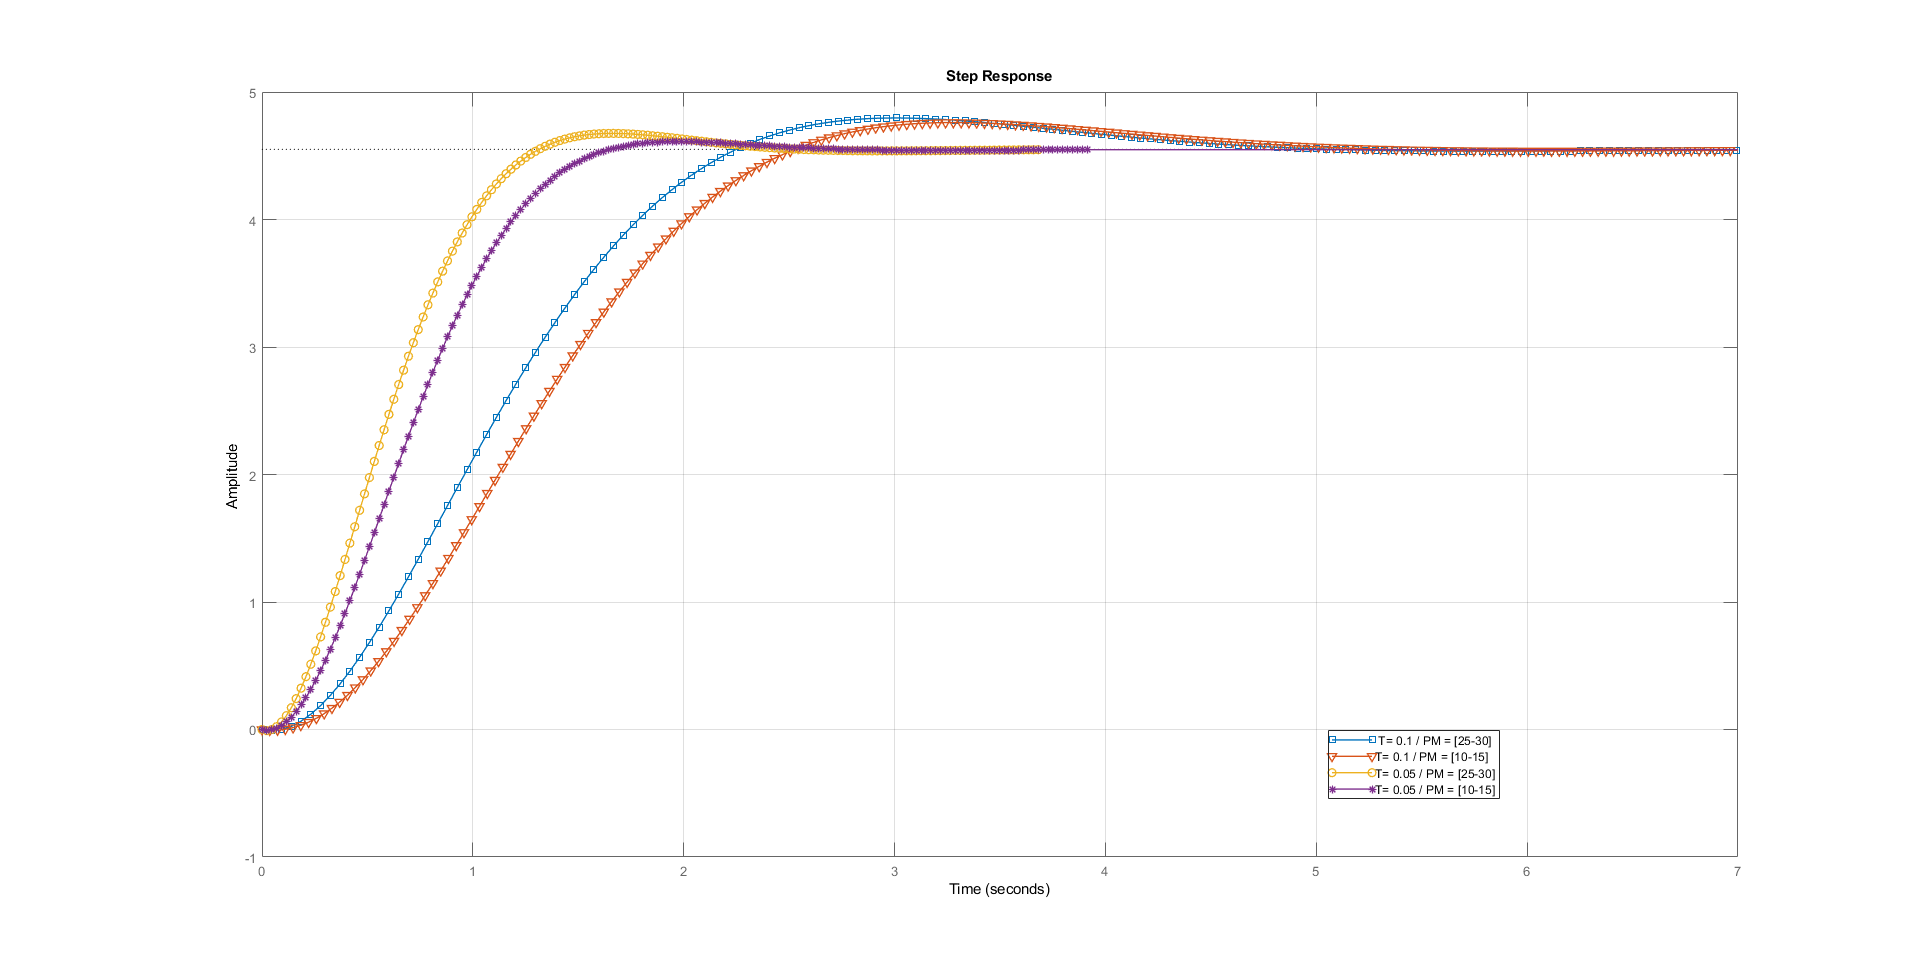
\includegraphics[width=1.0\unitlength]{images/final}
  		\caption{\label{fig:de} Difference in Step Responses of both compensated systems}
	\end{figure}
	
	As the phase margin is decreased the settling time is increased, the overshoot decreased. The steady state error stayed same. As the sampling time is increased from $T=0.05$ to $T=0.1$, the settling time again increased and the overshoot is decreased. The steady state error is not changed.
	
	
	
	
	
	
	
\newpage	 	
		 	

	
	
\end{enumerate}
	
%		\newpage
\begin{appendices}
	\section{Source Code For Matlab Parts}
		\lstinputlisting[language=Matlab]{MP5.m} \-\\[1cm]

%		\lstinputlisting[language=Matlab]{mydelta.m} \-\\[1cm]
%		\newpage
%	\section{Source Code For Question 3}
%		\lstinputlisting[language=Matlab]{q3.m} \-\\[1cm]
%	\section{Source Code For Question 4}
%		\lstinputlisting[language=Matlab]{q4.m} \-\\[1cm]
%				\lstinputlisting[language=Matlab,firstline=33, lastline=34]{q13.m} \-\\[1cm]
\end{appendices}
				

%\begin{appendices}
%\section{Source Code for Matlab Part}\label{appendix}
	%%	\lstinputlisting[language=Matlab,firstline=33, lastline=34]{q13.m} \-\\[1cm]		
%\lstinputlisting[language=Matlab]{Q1.m} 






\end{document}

%----samples------
%\begin{itemize}
%\item Item
%\item Item
%\end{itemize}

%\begin{figure}[H]
%\center
%\setlength{\unitlength}{\textwidth} 
%\includegraphics[width=0.7\unitlength]{images/logo1}
%\caption{\label{fig:logo}Logo }
%\end{figure}

%\begin{figure}[H]
%	\setlength{\unitlength}{\textwidth} 
%	\centering
%	\begin{subfigure}{.5\textwidth}
%  		\centering
%  		\includegraphics[width=0.48\unitlength]{images/logo1}
%  		\caption{\label{fig:logo1}Logo1 }
%	\end{subfigure}%
%	\begin{subfigure}{.5\textwidth}
%  		\centering
%		\includegraphics[width=0.48\unitlength]{images/logo2}
%  		\caption{\label{fig:logo2}Logo2}
%	\end{subfigure}
%\caption{\label{fig:calisandegree} Small Logos   }
%\end{figure}
	
%\begin{table}[H]
%  \centering
% 
%    \begin{tabular}{c|c|c}
%       $$A$$ & $$B$$ & $$C$$ \\ \hline
%       1 & 2 & 3  \\ \hline
%       2 & 3 & 4  \\ \hline
%       3 & 4 & 5  \\ \hline
%       4 & 5 & 6  
%      
%  \end{tabular}
%  \caption{table}
%  \label{tab:table}
%\end{table}
	
%\begin{table}[H]
%  \centering
% 
%    \begin{tabular}{c|c|c}
%       \backslashbox{$A$}{$a$} & $$\specialcell{ Average deviation \\ after subtracting out the  \\ frequency error }$$ & $$C$$ \\ \hline
%       \multirow{2}{*}{1} & 2 & 3  \\ \cline{2-3}
%        & 3 & 4  \\ \hline
%       3 & \multicolumn{2}{c}{4}  \\ \hline
%       4 & 5 & 6  
%      
%  \end{tabular}
%  \caption{table}
%  \label{tab:table}
%\end{table}
%-----end of samples-----